% Construction (repère mathématique) : arbre complet de hauteur 3.
%   Niveau 1 : (0, 2). Niveau 2 : (-1.6, 1), (1.6, 1).
%   Niveau 3 : (-2.4, 0), (-0.8, 0), (0.8, 0), (2.4, 0).
% SVG : x = 130 + 40x, y = 30 + 40(2 - y).
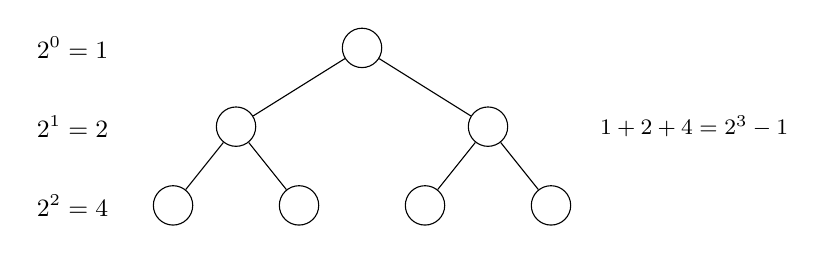
\begin{tikzpicture}[scale=1, every node/.style={font=\small}]
  \tikzstyle{n}=[draw, circle, inner sep=0pt, minimum size=5mm]
  \node[n] (a) at (0, 2) {};
  \node[n] (b) at (-1.6, 1) {}; \node[n] (c) at (1.6, 1) {};
  \node[n] (d) at (-2.4, 0) {}; \node[n] (e) at (-0.8, 0) {};
  \node[n] (f) at (0.8, 0) {};  \node[n] (g) at (2.4, 0) {};
  \draw (a) -- (b); \draw (a) -- (c);
  \draw (b) -- (d); \draw (b) -- (e); \draw (c) -- (f); \draw (c) -- (g);
  \node[left] at (-3.1, 2) {$2^0 = 1$};
  \node[left] at (-3.1, 1) {$2^1 = 2$};
  \node[left] at (-3.1, 0) {$2^2 = 4$};
  \node[right, font=\footnotesize] at (2.9, 1) {$1 + 2 + 4 = 2^3 - 1$};
\end{tikzpicture}
